\documentclass[tikz]{standalone}
\usepackage{amsmath,amssymb,xcolor}
\usetikzlibrary{arrows.meta,positioning,calc,backgrounds,fit}

% Colors
\colorlet{nodefill}{black!30}
\colorlet{nodedraw}{black!60}
\colorlet{solidedge}{black!70}
\colorlet{dashededge}{black!60}

% Styles and helpers
\newcommand\set[1]{\{#1\}}
\tikzset{
  setnode/.style={rounded corners=2pt, draw=nodedraw, fill=nodefill,
                  inner xsep=6pt, inner ysep=4pt, font=\footnotesize},
  startnode/.style={setnode, minimum width=8pt, inner sep=2pt},
  solidedge/.style={-Stealth, line width=1.2pt, draw=solidedge},
  dashededge/.style={-Stealth, dashed, line width=0.8pt, draw=dashededge},
  ann/.style={font=\footnotesize\itshape, text=dashededge, inner sep=1pt},
}

\begin{document}
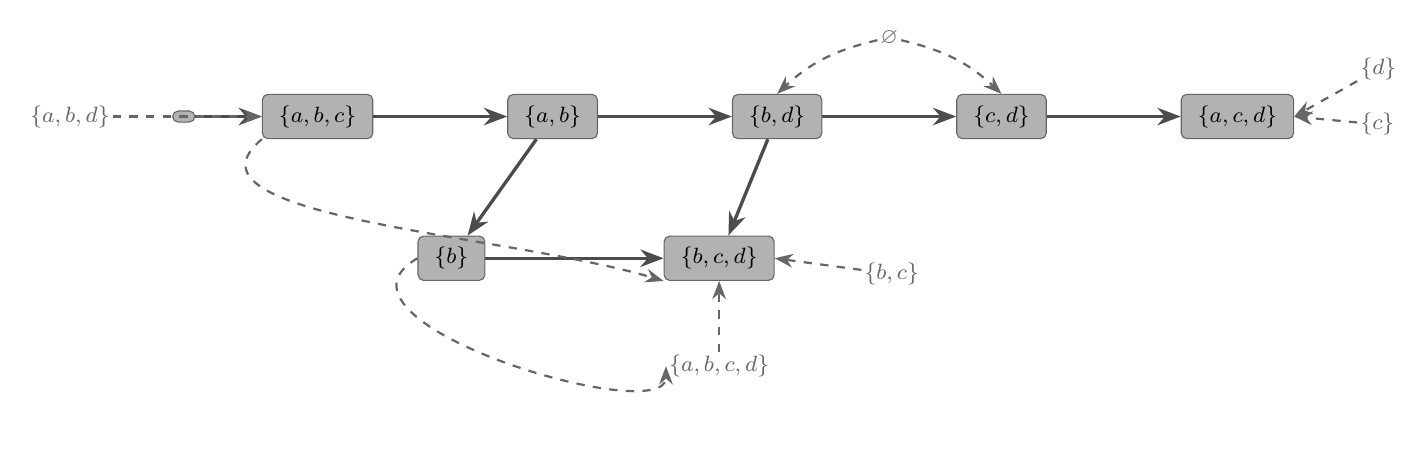
\begin{tikzpicture}[x=1cm,y=1cm,>=Stealth]

%--- Nodes (two rows) ----------------------------------------------------------
\node[startnode] (s0) at (-1.7, 0.9) {};

\node[setnode] (n1) at ( 0.0, 0.9) {$\set{a,b,c}$};
\node[setnode] (n2) [right=1.7 of n1] {$\set{a,b}$};
\node[setnode] (n3) [right=1.7 of n2] {$\set{b,d}$};
\node[setnode] (n4) [right=1.7 of n3] {$\set{c,d}$};
\node[setnode] (n5) [right=1.7 of n4] {$\set{a,c,d}$};

\node[setnode] (n6) at ( 1.7,-0.9) {$\set{b}$};
\node[setnode] (n7) at ( 5.1,-0.9) {$\set{b,c,d}$};

%--- Main (solid) arrows -------------------------------------------------------
\draw[solidedge] (s0) -- (n1);
\draw[solidedge] (n1) -- (n2);
\draw[solidedge] (n2) -- (n3);
\draw[solidedge] (n2) -- (n6);
\draw[solidedge] (n3) -- (n4);
\draw[solidedge] (n3) -- (n7);
\draw[solidedge] (n4) -- (n5);
\draw[solidedge] (n6) -- (n7);

%--- External annotations (dashed arrows) -------------------------------------
% left label -> n1
\node[ann, anchor=east] (L1) at (-2.6, 0.9) {$\set{a,b,d}$};
\draw[dashededge] (L1) -- (n1.west);

% top center empty set -> n3 and -> n4
\node[ann] (E) at ($(n3)!0.5!(n4)+(0,1.0)$) {$\varnothing$};
\draw[dashededge] (E) to[bend right=15] (n3.north);
\draw[dashededge] (E) to[bend left=15] (n4.north);

% right top labels -> n5
\node[ann, anchor=west] (Rd) at ($(n5.east)+(0.8,0.6)$) {$\set{d}$};
\node[ann, anchor=west] (Rc) at ($(n5.east)+(0.8,-0.1)$) {$\set{c}$};
\draw[dashededge] (Rd) -- (n5.east);
\draw[dashededge] (Rc) -- (n5.east);

% bottom center and right labels -> n7
\node[ann, anchor=north] (All) at ($(n7.south)+(0,-0.9)$) {$\set{a,b,c,d}$};
\draw[dashededge] (All) -- (n7.south);

\node[ann, anchor=west] (BC) at ($(n7.east)+(1.1,-0.2)$) {$\set{b,c}$};
\draw[dashededge] (BC) -- (n7.east);

% a few long dashed hints across the diagram (to mimic the original feel)
\draw[dashededge] (n1.south west) .. controls +(-1.2,-1.0) and +(-2.0,0.6) .. (n7.south west);
\draw[dashededge] (n6.west) .. controls +(-1.4,-0.8) and +(0,-0.8) .. (All.west);

\end{tikzpicture}
\end{document}